\documentclass[fleqn]{jbook}
\usepackage{physpub}

\begin{document}

\begin{question}{専攻 問題3}{}

スピン1の強磁性イジング模型
%
\[ {\cal H} = -\frac12 \sum_{i\neq j}J_{ij}I_iI_j + \sum_i DI_i^2%
    \hspace{10mm} (I_i,I_j=+1,0,-1) \]
%
を考える。ここで、$I_i$ は $i$ 番目の原子のスピン、$D$ は結晶場の効果を
表すパラメータ、$J_{ij}$ は $I_i$ と $I_j$ の間の交換相互作用であり、
最近接原子間では $J_{ij}=J(J>0)$、それ以外は $J_{ij}=0$ とする。
この系の相転移を分子場近似で考察する。各原子のまわりの最近接原子の数を
$z$ 、ボルツマン定数を $k$ とし、以下の問に答えよ。

\begin{subquestions}
\SubQuestion
  $i$ 番目の原子に着目すると、$I_i$ に対する有効ハミルトニアンは
  \[ {\cal H}_i = -B_{\rm eff} I_i + DI_i^2 \]
  と書ける。$i$ 以外の原子 $j$ のスピンの平均磁化 $M=<I_j>$ で置き
  換えたとき、$B_{\rm eff}$ を $z,J,M$ で表せ。さらに、$B_{\rm eff}$
  の物理的意味を記せ。

\SubQuestion
  ${\cal H}_i$ の固有値を用いて、温度 $T$ における $I_i$ の平均
  $\Mean{I_i}$ を $M$ で表せ。

\SubQuestion
  $\Mean{I_i}=M$ と置くことにより、$M$ を与える式が得られる。このとき、
  \begin{subsubquestions}
  \SubSubQuestion
    $D/(zJ) \rightarrow -\infty$
  \SubSubQuestion
    $D/(zJ) = 0$
  \SubSubQuestion
    $D/(zJ) \rightarrow +\infty$
  \end{subsubquestions}
  のそれぞれの場合について、$M=0$(常磁性状態)の他に$M\neq0$(強磁性状態)
  の解が存在するかどうかを議論し、存在する場合にはその臨界温度 $T_c$を
  求めよ。

\SubQuestion
  $D$ を $D=0$ から増加させると、ある臨界的な値 $D_t>0$ を境として、
  常磁性と強磁性間の相転移が二次から一次に変化する。そのような $D_t$と
  転移温度 $T_t$ を求めよ。(ヒント:$\Mean{I_i}$ を $M$ に関して3次
  まで展開し、その係数の符号を議論せよ。)

\SubQuestion
  横軸 $D$ 、縦軸 $T$ の平面における相図を図示せよ。ただし、境界を
  与える曲線の方程式などを具体的に求める必要はなく、非常に定性的な
  ものでよい。

\end{subquestions}
\end{question}
\begin{answer}{専攻 問題3}{}

\begin{subanswers}
\SubAnswer
  ${\cal H}$ から $I_i$ を含む部分だけを抜きだすと、
%
  \begin{equation}
    {\cal H}_i = -zJMI_i + DI_i^2    \eqname{1}
  \end{equation}
%
  よって$B_{\rm eff}=zJM$である。交換相互作用は本来電子間に働く
  クーロン力に由来するものだが、そのスピンに対する作用を磁場に
  換算した値が $B_{\rm eff}$ である。


\SubAnswer
  $I_i$の取り得る値は$-1,\,0,\,+1$であり、それぞれの起こる確率は
  $\exp{(-\beta{\cal H}_i})$に比例するので、よって$I_i$の平均値は
%
  \begin{eqnarray}
     \Mean{I_i}%
     &=& \frac{\sum_{I_i}I_ie^{-\beta{\cal H}_i}}%
         {\sum_{I_i}   e^{-\beta{\cal H}_i}}%
      =  \frac{-e^{-\beta(+zJM+D)}+e^{-\beta(-zJM+D)}}%
         {e^{-\beta(+zJM+D)}+e^{0}+e^{-\beta(-zJM+D)}}%
         \nonumber\\
     &=& \frac{e^{-\beta D}(e^{+\beta zJM}-e^{-\beta zJM})}%
         {1+e^{-\beta D}(e^{+\beta zJM}+e^{-\beta zJM})}
      =  \frac{2\sinh(\beta zJM)}{e^{\beta D} + 2\cosh(\beta zJM)}
    \eqname{2}
  \end{eqnarray}
%

\SubAnswer
  \begin{subsubanswers}
  \SubSubAnswer
    $D/(zJ)\rightarrow -\infty$ のとき、式\eqhref{1}よりスピンが
    大きい方が安定なので
    強磁性になる傾向が強いと考えられる。
    \eqhref{2}式は次式となる。
%
    \[ \Mean{I_i} = \tanh(\beta zJM) \]
%
    $\Mean{I_i}$は、$M$ について単調増大し、また十分大きい $M$ に
    対しては $\Mean{I_i}<M$ となるから、$M=0$ 以外で $\Mean{I_i}=M$
    となるような $M$ が存在するのは、$\Mean{I_i}$ の原点での傾きが $M$ 
    の原点での傾きより大きいときである。よって、
%
    \[ \Partial{}{M}\tanh(\beta zJM)\Bigr|_{M=0} > 1%
       \qquad\Yueni%
       \beta zJ > 1%
       \qquad\Yueni%
       T<\frac{zJ}{k} \;(= T_c) \]
%

  \SubSubAnswer
    $D/(zJ)=0$ のとき、式\eqhref{1}より、強磁性は起こり得るが、
    (i)の場合ほどではない。
    式\eqhref{2}は次式となる。
%
    \[ \Mean{I_i} = \frac{2\sinh(\beta zJM)}{1+2\cosh(\beta zJM)} \]
%
    この $\Mean{I_i}$ も (i) のものと同様に振舞うから、
%
    \[ \Partial{\Mean{I_i}}{M}\Bigr|_{M=0}%
       = \beta zJ \frac{2\cosh(\beta zJM)+4}%
                       {(1+2\cosh(\beta zJM))^2} \Bigr|_{M=0}%
       = \frac{2}{3} \beta zJ > 1%
       \qquad\Yueni%
       T<\frac{2zJ}{3k} \;(=T_c) \]
%

  \SubSubAnswer
    $D/(zJ)\rightarrow+\infty$ のとき、式\eqhref{1}より、スピンの
    大きさが$0$の方が安定なので強磁性は起こらない。
    実際、式\eqhref{2}は $\Mean{I_i} = 0$となり、これは $M=0$ にしか
    解を持たない。

  \end{subsubanswers}

\SubAnswer
  $x\equiv \beta zJM$、 $y\equiv \beta zJ\Mean{I_i}$として
  式\eqhref{2}を書き直すと
%
  \[ y = \beta zJ \frac{2\sinh{x}}{e^{\beta D}+2\cosh{x}} \]
%
  $x\ll 1$の範囲でこの式の右辺を展開する。
%
  \begin{eqnarray}
     y &\simeq& 2\beta zJ \frac{x+x^3/6}{e^{\beta D}+2+x^2}%
       =      \frac{2\beta zJ}{e^{\beta D}+2}%
              \Bigl(x+\frac{x^3}{6}\Bigr)%
              \Bigl(1+\frac{x^2}{e^{\beta D}+2}\Bigr)^{-1} \nonumber\\
       &\simeq& \frac{2\beta zJ}{e^{\beta D}+2}%
              \Bigl[%
                x+\Biggl(\frac{1}{6}-\frac{1}{e^{\beta D}+2}\Biggr)x^3%
              \Bigr] \eqname{3}
  \end{eqnarray}
%
  この$y$が$x$に等しくなる$x$の解を求めるわけである。\\
%
\newpage
  式\eqhref{3}の$x$の$3$次の項の係数が負である場合の
  $T>T_c,\,T=T_c,\,T<T_c$の3種類の温度での$x,y$のグラフを下の左図に示す。
  このように、この時の相転移点において解の$x$が連続である。よって
  2次相転移である。\\
%
  他方、式\eqhref{3}の$x$の$3$次の項の係数が正である場合の
  $T>T_c,\,T=T_c,\,T<T_c$の3種類の温度での$x,y$のグラフを下の右図に示す。
  このように、この時の相転移点において解の$x$が不連続である。よって
  1次相転移である。
%
  \begin{center}
    \mbox{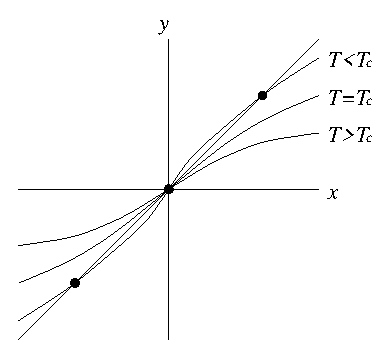
\includegraphics[clip]{1993phy3-1.eps}}\hspace{15mm}
    \mbox{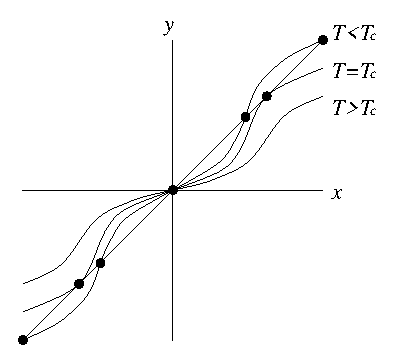
\includegraphics[clip]{1993phy3-2.eps}}
  \end{center}
%
  このように相転移の種類が変わる敷居は式\eqhref{3}の$x$の$3$次の
  項の係数が$0$になる所であり、またこの場合には相転移が起こる温度は
  式\eqhref{3}の$x$の$1$次の項の係数が$1$になる所である。すなわち、
%
  \[ \frac{1}{6}-\frac{1}{e^{\beta D}+2} = 0 \hspace{20mm}%
     \frac{2\beta zJ}{e^{\beta D}+2} = 1 \]
%
  これらを満たす$D,\beta$が求める$D_t,\,T_t$である。
%
  \[ D_t = \frac{zJ}{3}\ln4  \hspace{10mm}%
     T_t = \frac{zJ}{3k} \]
%


\SubAnswer
  $D=0,\pm\infty$ の場合については既に求めた。
  $0<D<\infty$ のどこかで、$M=\Mean{I_i}$ が原点以外に解を持たなくなる
  ような $D$が存在するはずで、相図は下のようになると考えられる。
  (para:常磁性、ferro:強磁性)
%
  \begin{center}
    \mbox{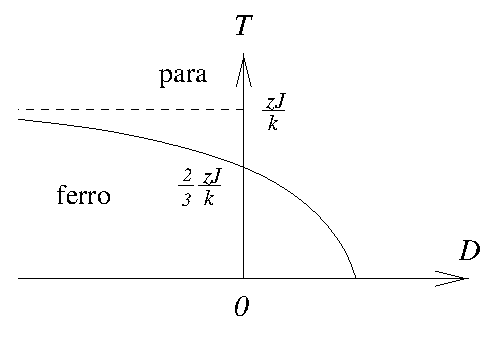
\includegraphics[clip]{1993phy3-3.eps}}
  \end{center}

\end{subanswers}
\end{answer}


\end{document}
